\documentclass[journal]{../IEEEtran}

\usepackage{graphicx}
\usepackage{fancyhdr}
\usepackage{epsfig} % for postscript graphics files
\usepackage{graphics} % for pdf, bitmapped graphics files

\graphicspath{{Figures/}}

\pagestyle{fancy}
\lhead{CPE 470/670}
\rhead{\thepage}
\chead{Team 6: Lab 7 Report}
\lfoot{}
\rfoot{}
\cfoot{}

\begin{document}

\begin{titlepage}
    \vspace*{\fill}
    \begin{center}
      {\LARGE \bf Lab 7: Soccer Robot}

      {Team 6: Alexander  C. Woods and Taylor Mansfield}

      November 5, 2014
    \end{center}
    \vspace*{\fill}
  \end{titlepage}


\section{Hardware and Software Design}\label{S.design}
\IEEEPARstart{P}{laying} soccer with a robot is a fun and interesting challenge. The robot must be able to sense the location of the ball, determine whether or not it should be attacking or defending, and act accordingly. The field on which the robots played is shown in Fig.~\ref{F.field}. The field consists of a goal on each end, which span the entire width. The goals are marked by black zones and the ball must completely enter the zone in order to be considered a point.

%\begin{figure}[ht]
%\centering
%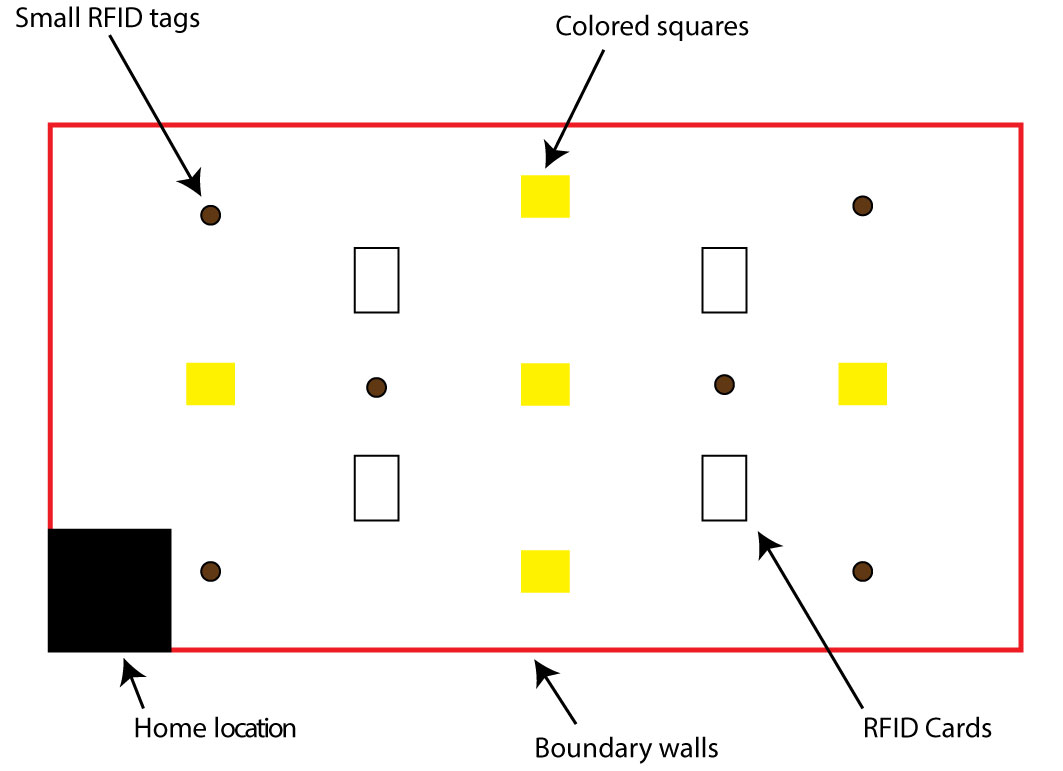
\includegraphics[width=1\columnwidth]{field.jpg}\\
%\caption{The field on which the robots play soccer has a goal on each end which spans the width of .}
%\label{F.ramp}
%\end{figure}

The sensors used for this challenge are quite simple. An IR sensor is used to detect the location of the ball according to the map shown in Fig.~\ref{F.ir_map.eps}. The only other sensor used in this challenge is a compass sensor which is used to determine the heading of the 

An ultrasonic sensor is equipped which lets the robot sense and avoid wall while it is looking for balls. The ultrasonic sensor is strategically located on the left side of the robot as shown in Fig.~\ref{F.us_sensor} so that it can sense walls, but will not be fooled by a ball. This is because the robot keeps the wall on its left side naturally. If the robot were to use a right sided wall following technique instead the ultrasonic sensor would be located on the other side of the robot.

\section{Problems Encountered}\label{S.problems}



\section{Solutions}\label{S.solutions}



\section{Unsolved Problems}\label{S.unsolved}



\end{document}
